\documentclass[12pt]{article}

\pdfoutput=1
\usepackage{hyperref}
\usepackage{epstopdf}
%\usepackage{fullpage}
\usepackage{amssymb}
\usepackage{amsmath}
\usepackage{color}
\usepackage{graphicx}
\usepackage{caption}
\usepackage{subcaption}
%\usepackage{boondox-cal}%for calligraphic font
%\usepackage{kbordermatrix}
%\usepackage{algpseudocode}
%\usepackage{algorithm}

%\usepackage{apacite}

\title{Synthetic data}
\author{Arash Khodadadi}

\begin{document}
\maketitle

\section{Introduction}

To analyze the proposed optimization methods, we first fit the model on some synthetic spatio-temporal data. The observations at all time steps and all locations were generated from independent Gaussian random variables with zero mean. However, the variance of these random variables changes smoothly in time and space. Specifically, the observation at time step $t$ and at location $(r,c)$ on the grid is generated from a Gaussian $N(0,\sigma^2(t,r,c))$, where:

\begin{equation}
\begin{aligned}
\sigma(t,r,c) & =\sum_{s=1}^{S} W_s(t) \cdot \exp\bigg( \frac{(r-r_s)^2+(c-c_s)^2}{2\sigma_s^2} \bigg) \\
W_s(t) & =\alpha_s \cdot t + \exp(\sin(2\pi\omega_s t+\phi_s)) 
\label{eq:sourceVar}
\end{aligned}
\end{equation}

In words, the variance at each time and location is computed as the weighted sum of $S$ bell-shaped functions where the weights are time-varying functions. Specifically, the weights consist of a linear trend $\alpha_s \cdot t$ and a periodic term $\beta_s \cdot \sin(2\pi\omega_s t+\phi_s)$. The bell-shaped functions impose the spatial smoothness, and the linear trend and the periodic terms enforce the temporal smoothness. We simulated the data on a 5 by 7 grid and for 780 time steps. We also used $S=4$. The parameters of the variance function are shown in Table \ref{tab:sim_params}. The value of the variance function for all locations on the grid and at $t=25$ and $t=45$ is shown in Figure \ref{fig:true_var_spatial}. Also, the variance for all time steps and at the location (0,0) on the grid is shown in Figure \ref{fig:true_fitted_var}. The linear trend and the period term can be seen clearly in this figure.

\begin{table}[t]
	\caption{Parameters used to simulate data}
	\label{tab:sim_params}
	\vskip 0.15in
	\begin{center}
		\begin{small}
			\begin{sc}
				\begin{tabular}{ccccccc}
					\hline

					$s$ & $r_s$ & $c_s$ & $\sigma_s$ &$\alpha_s$ & $\omega_s$ & $\phi_s$\\
					\hline
					1 & 0 & 0 & 5 & 0.5 & 0.121 & 0 \\
					2 & 0 & 5 & 5 & 0.1 & 0.121 & 0 \\
					3 & 3 & 0 & 5 & -0.5 & 0.121 & $\pi/2$ \\
					4 & 3 & 5 & 5 & -0.1 & 0.121 & $\pi/2$ \\
					\hline
				\end{tabular}
			\end{sc}
		\end{small}
	\end{center}
	\vskip -0.1in
\end{table} 

\begin{figure}[!h]
	\centering	
	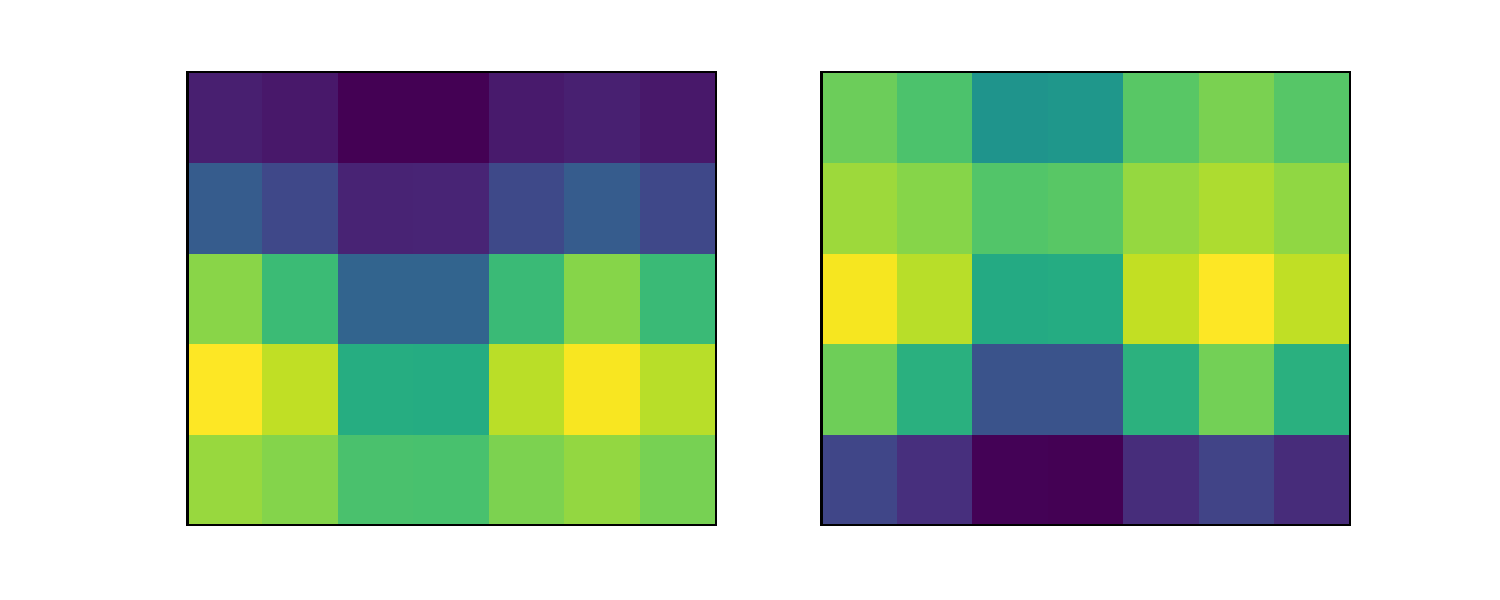
\includegraphics[width=.7\linewidth]{Figures/true_var_spatial}		
	
	\caption{{\bf Variance function at $t=25$ (left) and $t=45$ (right)}} \label{fig:true_var_spatial}
\end{figure}

\section{Convergence}
Figure \ref{fig:convergence} shows the convergence of the two algorithms. Each iteration of the linearized algorithm takes about 0.01 seconds on average while each iteration of the consensus ADMM takes about 20 seconds. 

\begin{figure}[!h]
	\centering	
	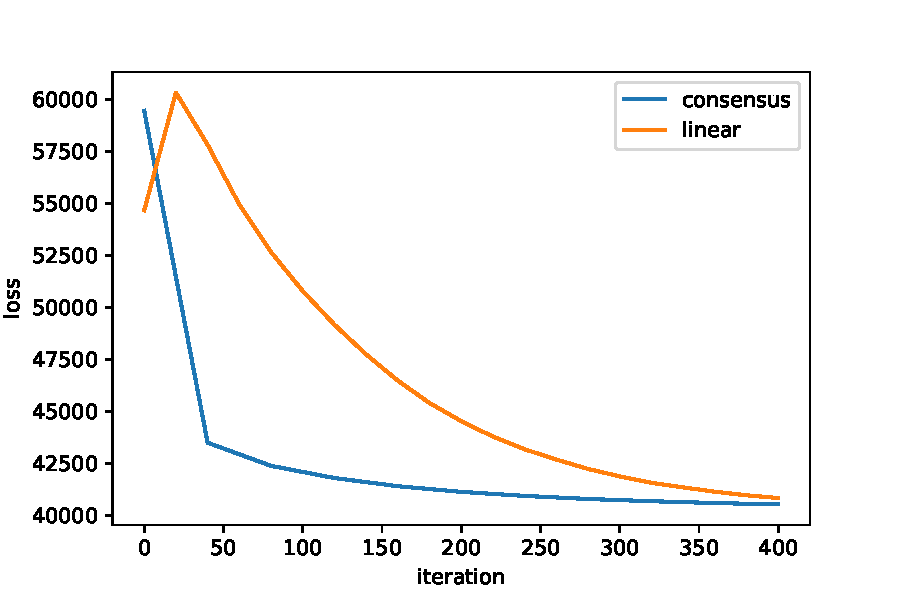
\includegraphics[width=.7\linewidth]{Figures/convergence}		
	
	\caption{{\bf Convergence of linearized and consensus ADMM.}} \label{fig:convergence}
\end{figure}

\section{Model selection}
We fitted the linearized ADMM for all combinations of values of $\lambda_t$ and $\lambda_s$ from the sets $\lambda_t \in \{0,1,5,10,50,100\}$ and $\lambda_s \in \{0,0.05,0.1,0.2,0.3\}$. For each pair, we then compute the mean absolute error (MAE) between the estimated variance and the true variance at all locations and all time steps. For $\lambda_t=5$ and $\lambda_s=0.1$ MAE was minimized. Figure \ref{fig:true_fitted_var} shows the true and the estimated standard deviation at location (0,0) using $\lambda_s=0.1$ and $\lambda_t=5$ (blue) and $\lambda_t=100$ (green). As we can see, larger than optimal value of $\lambda_t$ leads to estimated values which are ``too smooth".

\begin{figure}[!h]
	\centering	
	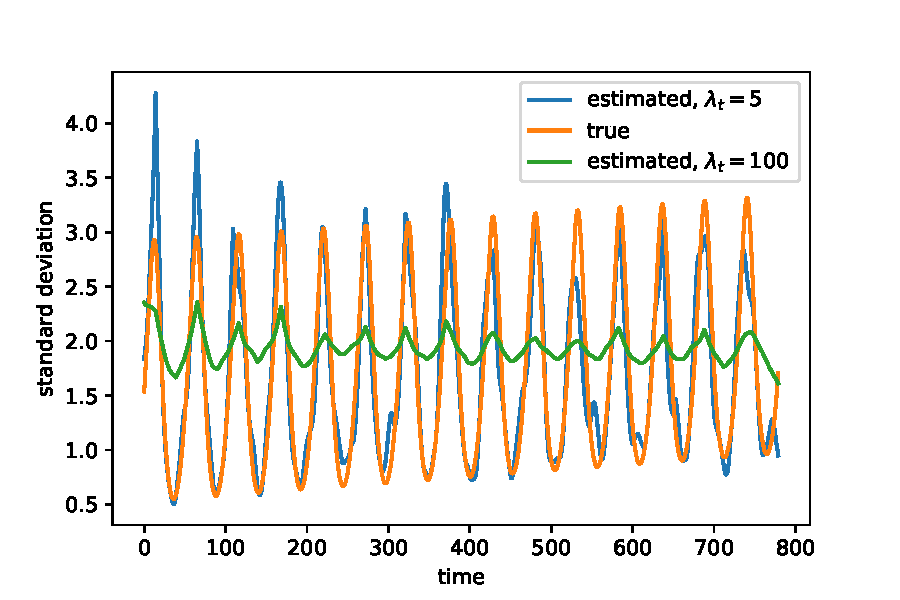
\includegraphics[width=.7\linewidth]{Figures/true_fitted_var}		
	
	\caption{{\bf The true (orange) and estimated standard deviation function at the location (0,0). The estimated values are obtained using linearized ADMM with $\lambda_s=0.1$ and two values of $\lambda_t$: $\lambda_t=5$ (blue) and $\lambda_t=100$ (green).}} \label{fig:true_fitted_var}
\end{figure}

\bibliographystyle{unsrt}
\bibliography{references}

\end{document}